\documentclass[a4paper,14pt]{extarticle}
\usepackage[utf8]{inputenc}
\usepackage[english,russian]{babel}

\usepackage{amsthm}
\usepackage{graphicx}
\usepackage{caption}
\usepackage{amssymb}
\usepackage{amsmath}
\usepackage{mathrsfs}
\usepackage{euscript}
\usepackage{graphicx}
\usepackage{subfig}
\usepackage{caption}
\usepackage{color}
\usepackage{bm}
\usepackage{tabularx}
\usepackage{adjustbox}


\usepackage[toc,page]{appendix}

\usepackage{comment}
\usepackage{rotating}

\DeclareMathOperator*{\argmax}{arg\,max}
\DeclareMathOperator*{\argmin}{arg\,min}

\newtheorem{theorem}{Теорема}
\newtheorem{lemma}[theorem]{Лемма}
\newtheorem{definition}{Определение}[section]

\numberwithin{equation}{section}

\newcommand*{\No}{No.}

\begin{document}

% Титульный лист
%\input{./frontpage.tex}

% Аннотация
\newpage


\begin{abstract}
Исследуется проблема понижения сложности аппроксимирующей модели при переносе на новые данные меньшей мощности. Вводятся понятия учителя, ученика для разных наборов данных. При этом мощность одного набора данных больше мощности другого. Рассматриваются методы, основанные на дистилляции моделей машинного обучения. Вводится предположение, что решение оптимизационной задачи от параметров обеих моделей и доменов повышает качество модели ученика. Проводится вычислительный эксперимент на реальных и синтетических данных.


\smallskip
\textbf{Ключевые слова}: адаптация доменов, дистилляция, нейронные сети, обучение с учителем
\end{abstract}


% Нумерация должна начинаться со второй страницы
\setcounter{page}{2}

% Оглавление
\newpage
\tableofcontents


% Введение
\newpage


\section{Введение}


\section{Анализ литературы}

В ~\cite{Hinton2015} рассматривается метод учета меток учителя, используя функцию softmax с параметром температуры.\\
В ~\cite{Vapnik2016} рассматривается метод дистилляции в случае несовпадения признаковых описаний ученика и учителя\\


% Введение
\newpage

\section{Постановка задачи}

\subsection{Базовая постановка задачи дистилляции}

Задана выборка 
$$\mathfrak{D}=(\mathbf{X},\mathbf{Y}), \quad \mathbf{X} \in \mathbb{X},
\quad \mathbf{Y} \in \{1,...,R\},$$
где $R$ --- число классов в задаче классификации.

Предполагается, что задана обученная модель с большим числом параметров --- модель учителя. Модель учителя $\mathbf{f}$ принадлежит параметрическому семейству функций: $$\mathfrak{F}=\{\mathbf{f}|\mathbf{f}=\text{softmax}(\mathbf{v(x)}/T), \mathbf{v}:\mathbb{R}^{n}\rightarrow \mathbb{R}^{R}\}.$$

Требуется обучить модель ученика с меньшим числом параметров с учетом ответов учителя. Модель ученика $\mathbf{g}$ принадлежит параметрическому семейству функций: $$\mathfrak{G}=\{\mathbf{g}|\mathbf{g}=\text{softmax}(\mathbf{z(x)}/T), \mathbf{z}:\mathbb{R}^{n}\rightarrow \mathbb{R}^{R}\},$$
где $\mathbf{v, z}$ --- дифференцируемые параметрические функции заданной структуры, $T$ --- параметр температуры со свойствами:
\begin{enumerate}
    \item при $T \rightarrow 0$ один из классов имеет единичную вероятность;
    \item при $T \rightarrow \infty$ все классы равновероятны.
\end{enumerate}

Функция потерь $\mathcal{L}$, учитывающая модель учителя $\mathbf{f}$ при выборе модели ученика $\mathbf{g}$, имеет вид:
\[
\begin{aligned}
    \mathcal{L}(\mathbf{w,X,Y,f})=&-\sum\limits_{i=1}^{m}\sum\limits_{r=1}^{R}y_{i}^{r}\log{g^{r}(x_{i})}\bigr|_{T=1}\\
    &-\sum\limits_{i=1}^{m}\sum\limits_{r=1}^{R}f^{r}(x_{i})\bigr|_{T=T_{0}}\log{g^{r}(x_{i})}\bigr|_{T=T_{0}},
\end{aligned}
\]
где $\cdot\bigr|_{T=t}$ означает, что параметр температуры $T$ в предыдущей функции равен $t$.

Получаем оптимизационную задачу:
$$\hat{\mathbf{w}} = \arg\min_{\mathbf{w} \in \mathbb{W}} \mathcal{L}(\mathbf{w,X,Y,f}).$$


\subsection{Постановка задачи дистилляции для многодоменной выборки}

Заданы две выборки:
$$\mathfrak{D}_{\text{s}}=(\mathbf{X}_{\text{s}},\mathbf{Y}_{\text{s}}),
\quad \mathbf{X}_{\text{s}} \in \mathbb{X}_{\text{s}},
\quad \mathbf{Y}_{\text{s}} \in \mathbb{Y}$$
$$\mathfrak{D}_{\text{t}}=(\mathbf{X}_{\text{t}},\mathbf{Y}_{\text{t}}), \quad \mathbf{X}_{\text{t}} \in \mathbb{X}_{\text{t}},
\quad \mathbf{Y}_{\text{t}} \in \mathbb{Y},$$
где $\mathfrak{D}_{\text{s}}, \mathfrak{D}_{\text{t}}$ --- исходный и целевой наборы данных. В базовой постановке задачи дистилляции предполагается, что 
$\mathfrak{D}_{\text{t}} \subset \mathfrak{D}_{\text{s}},
\mathbb{X}_{\text{t}}=\mathbb{X}_{\text{s}}$.

Предполагается, что число объектов в выборках не совпадают:
$$|\mathbf{X}_{\text{s}}| \gg |\mathbf{X}_{\text{t}}|$$

Пусть при этом задана модель учителя на выборке большей мощности:
$$\mathbf{f}: \mathbb{X}_{\text{s}} \rightarrow \mathbb{Y}^{\prime},$$
где $\mathbf{f}$ --- модель учителя, $\mathbb{Y}^{\prime}$ --- пространство оценок.

Задана связь между исходной и целевой выборками:
$$\varphi: \mathbb{X}_{\text{t}} \rightarrow \mathbb{X}_{\text{s}},$$
где $\varphi$ ---  инъективное отображение.

Требуется получить модель ученика для малоресурсной выборки:
$$\mathbf{g}: \mathbb{X}_{\text{t}} \rightarrow \mathbb{Y}^{\prime},$$
где $\mathbf{g}$ --- модель ученика.

В работе рассматривается функция потерь, учитывающая метки учителя и связь между доменами:
\begin{enumerate}
    \item для задачи регрессии:
    \[
    \begin{aligned}
    \mathcal{L}(\mathbf{w,X,Y,f,\varphi})=&\lambda\|\mathbf{y}-\mathbf{g}(\mathbf{x},\mathbf{w})\|_{2}^{2}\\
    &+(1-\lambda)\|\mathbf{g}(\mathbf{x},\mathbf{w})-(\mathbf{f}\circ \mathbf{\varphi})(\mathbf{x})\|_{2}^{2};
    \end{aligned}
    \]
    \item для задачи классификации:
    \[
    \begin{aligned}
    \mathcal{L}(\mathbf{w,X,Y,f,\varphi})=&-\lambda\sum\limits_{i=1}^{m}\sum\limits_{r=1}^{R}\mathbb{I}[y_{i}=r]\log{g^{r}(\mathbf{x}_{i},\mathbf{w})}\\
    &-(1-\lambda)\sum\limits_{i=1}^{m}\sum\limits_{r=1}^{R}(f\circ \varphi)^{r}(\mathbf{x}_{i})\log{g^{r}(\mathbf{x}_{i},\mathbf{w})},
    \end{aligned}
    \]
    где $\lambda$ --- метапараметр, задающий вес дистилляции, $\mathbb{I}$ --- индикаторная функция.
\end{enumerate}

Получаем оптимизационную задачу:
$$\hat{\mathbf{w}} = \arg\min_{\mathbf{w} \in \mathbb{W}} \mathcal{L}(\mathbf{w,X,Y,f,\varphi}).$$



% Введение
\newpage

\section{Вычислительный эксперимент}

Для анализа моделей, полученных путем дистилляции модели учителя в модель ученика, проводится вычислительный эксперимент для задачи классификации.\\
Эксперимент проводится для выборки FashionMNIST~\cite{FMNIST} - набора изображений предметов одежды. В качестве моделей учителя $\textbf{f}$ и ученика $\textbf{g}$ рассматриваются четырёхслойная и однослойная нейронные сети соответсвенно. Для решения оптимизационной задачи используется Adam, функция активации - ReLu.\\
Выборка разделяется на 3 части: две для обучения многоресурного и малоресурсного доменов, а также тестовая часть выборки. Многоресурсная часть содержит 59000 объектов, малоресурсная часть содержит 1000 объектов, а тестовая часть содержит 10000 объектов.
\newpage
\subsection{Анализ дистилляции Хинтона}

\paragraph{Обучение на обоих доменах.}
Модель учителя и ученика обучаются на обоих доменах.\\
На рис.1а показан график зависимости метрики accuracy на тестовой выборке между истинными метками объектов и вероятностями, предсказанными моделью ученика.\\
На рис.1б показан график зависимости кросс-энтропии на тестовой выборке между истинными метками объектов и вероятностями, предсказанными моделью ученика.\\
На графиках видно, что модель, использующая метки учителя, показывает лучшее значение accuracy, при этом наблюдается значительное снижение ошибки.
\begin{figure}[h!t]\center
\subfloat[]
{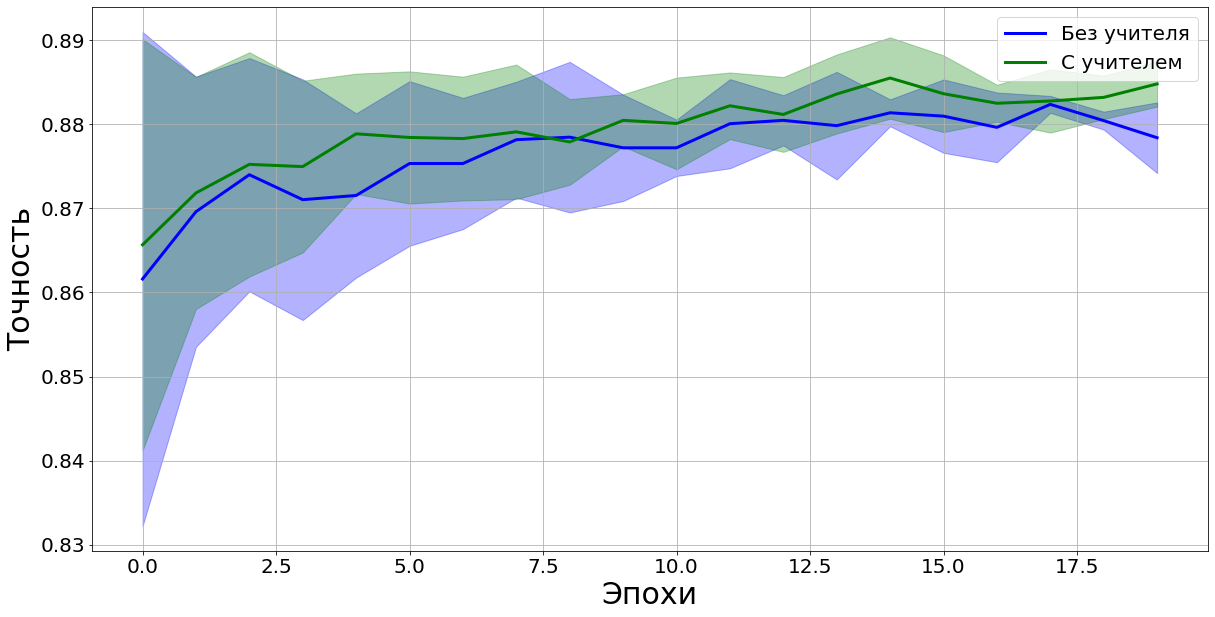
\includegraphics[width=0.5\textwidth]{results/acc}}
\subfloat[]
{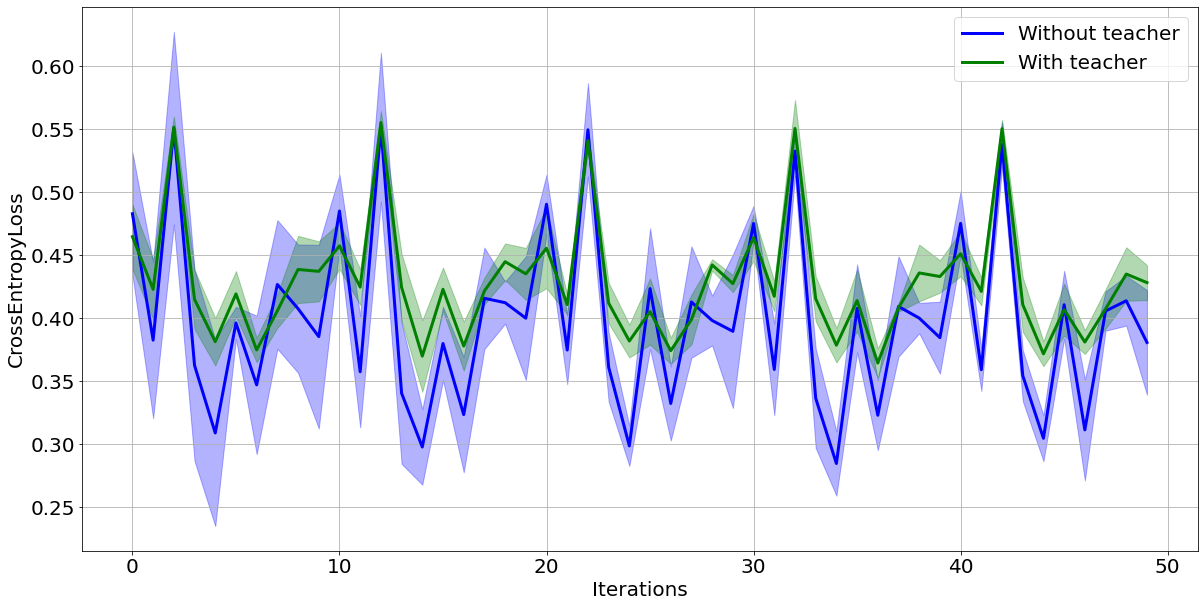
\includegraphics[width=0.5\textwidth]{results/loss}}\\
\caption{Качество аппроксимации на тестовой выборке a) accuracy; b) CrossEntropyLoss между истинными и предсказанными учеником метками}
\end{figure}

\newpage
\paragraph{Обучение на малоресурсном домене.}
Модель учителя обучается на многоресурсном домене, а модель ученика обучается на малоресурсном домене.\\
На рис.2а показан график зависимости метрики accuracy на тестовой выборке между истинными метками объектов и вероятностями, предсказанными моделью ученика.\\
На рис.2б показан график зависимости кросс-энтропии на тестовой выборке между истинными метками объектов и вероятностями, предсказанными моделью ученика.\\
На графиках видно, что модель, использующая метки учителя, показывает лучшее значение accuracy, при этом наблюдается снижение ошибки.
\begin{figure}[h!t]\center
\subfloat[]
{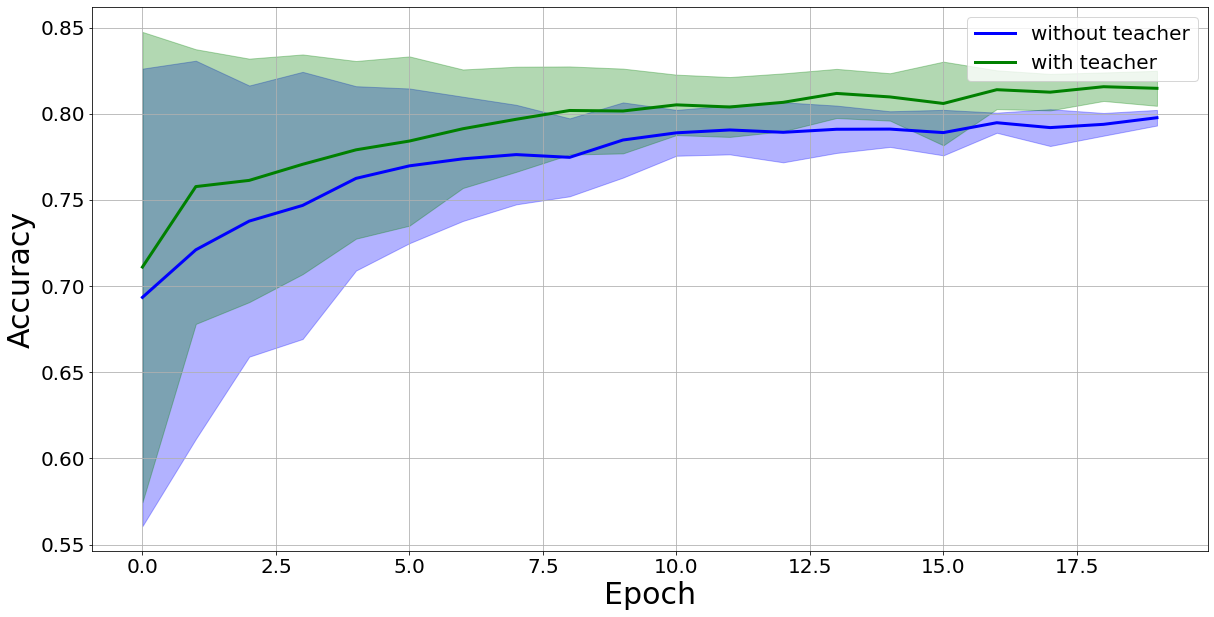
\includegraphics[width=0.5\textwidth]{results/small_acc}}
\subfloat[]
{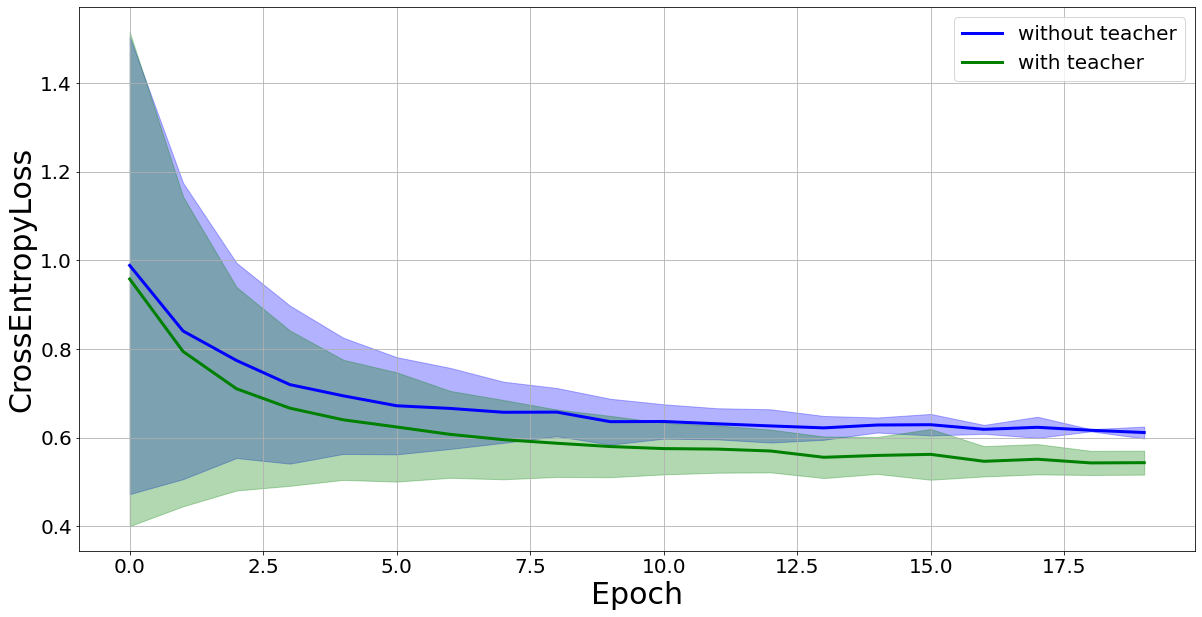
\includegraphics[width=0.5\textwidth]{results/small_loss}}\\
\caption{Качество аппроксимации на тестовой выборке a) accuracy; b) CrossEntropyLoss между истинными и предсказанными учеником метками}
\end{figure}

\newpage
\paragraph{Обучение на выборке с шумом.}
Добавим к многоресурсному домену нормальный шум $\mathcal{N}(0,0.08)$ и обучим на нем модель учителя. Модель ученика обучается на малоресурсном домене.
\begin{figure}[h!t]\center
{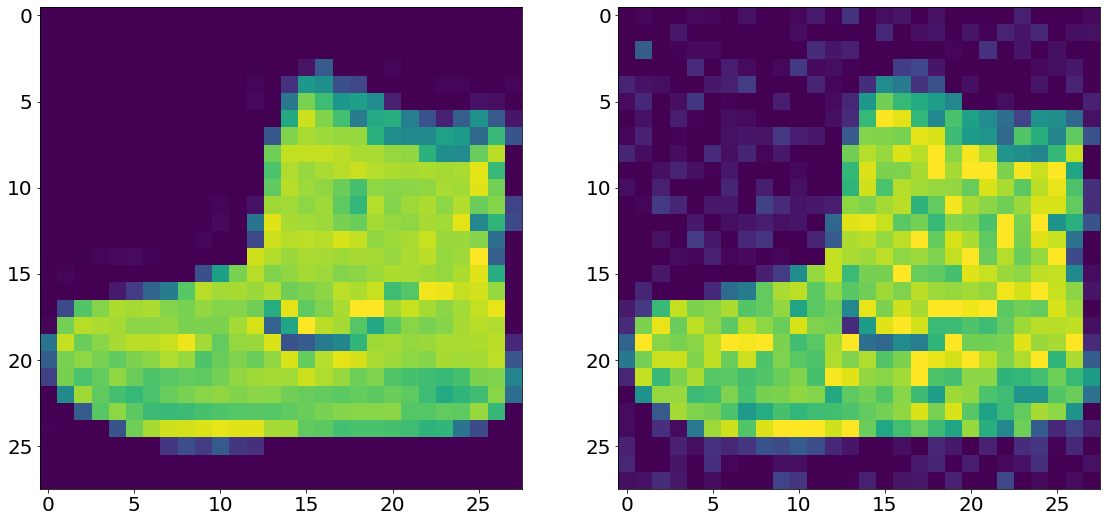
\includegraphics[width=0.5\textwidth]{results/noise}}
\caption{Сравнение объекта выборки до и после добавления шума}
\end{figure}\\
На рис.4а показан график зависимости метрики accuracy на тестовой выборке между истинными метками объектов и вероятностями, предсказанными моделью ученика.\\
На рис.4б показан график зависимости кросс-энтропии на тестовой выборке между истинными метками объектов и вероятностями, предсказанными моделью ученика.\\
На графиках видно, что значения accuracy и CrossEntropyLoss модели, использующей метки учителя на выборке с шумом, лежат между соответствующими значениями для модели без учителя и для модели, использующей метки учителя на выборке без шума.

\begin{figure}[h!t]\center
\subfloat[]
{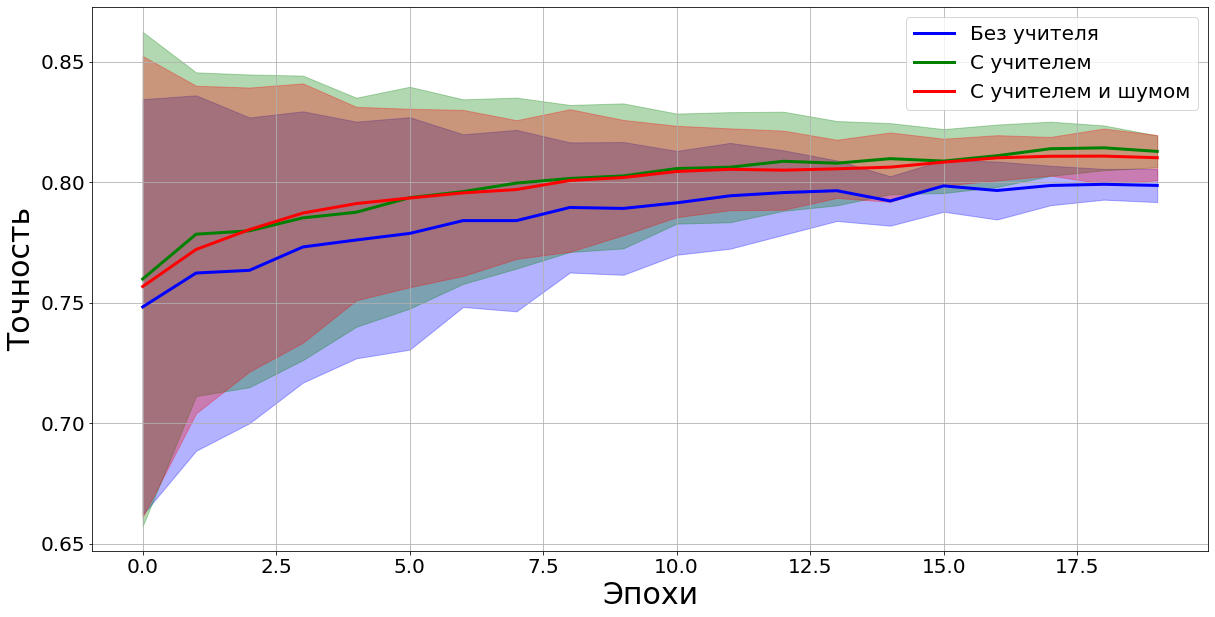
\includegraphics[width=0.5\textwidth]{results/noise_acc}}
\subfloat[]
{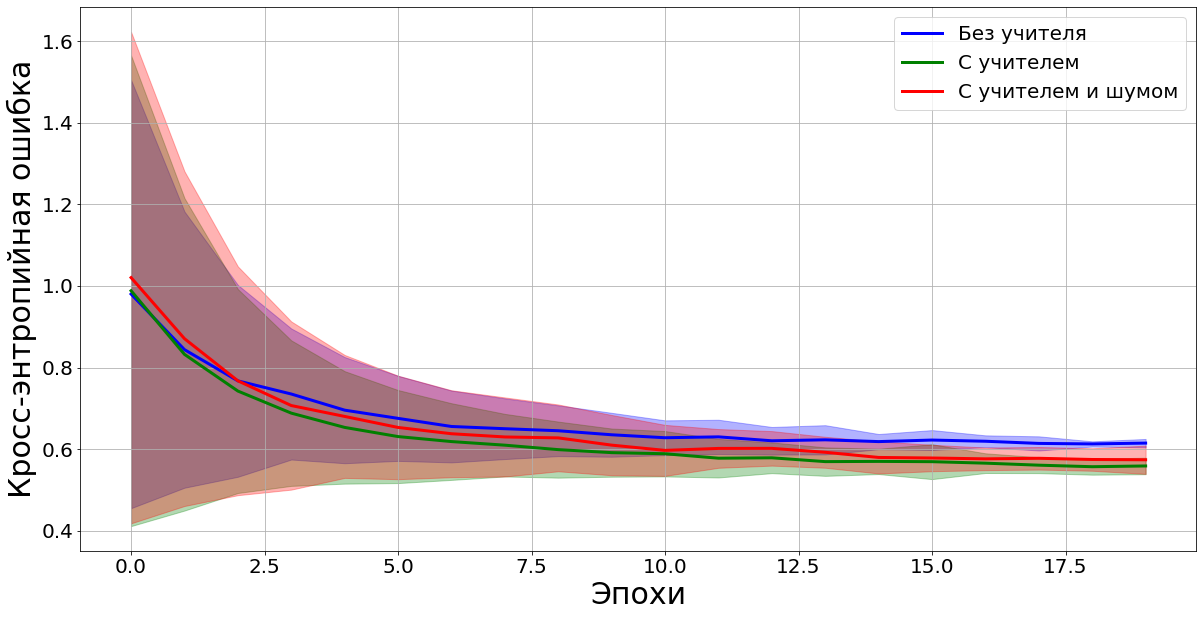
\includegraphics[width=0.5\textwidth]{results/noise_loss}}\\
\caption{Качество аппроксимации на тестовой выборке a) accuracy; b) CrossEntropyLoss между истинными и предсказанными учеником метками}
\end{figure}

\paragraph{Обучение на выборке с dilation.}
Применим к многоресурсному домену сверточное преобразование с параметром $\text{dilation}=2$ и обучим на нем модель учителя. Модель ученика обучается на малоресурсном домене.\\
\begin{figure}[h!t]\center
{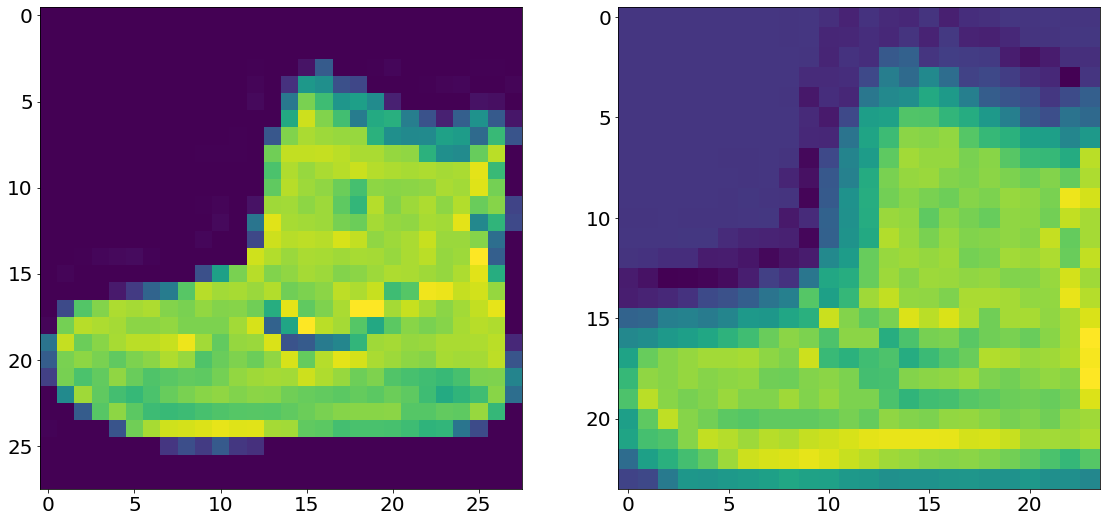
\includegraphics[width=0.5\textwidth]{results/dilation}}
\caption{Сравнение объекта выборки до и после преобразования}
\end{figure}\\
На рис.6а показан график зависимости метрики accuracy на тестовой выборке между истинными метками объектов и вероятностями, предсказанными моделью ученика.\\
На рис.6б показан график зависимости кросс-энтропии на тестовой выборке между истинными метками объектов и вероятностями, предсказанными моделью ученика.\\
На графиках видно, что значения accuracy и CrossEntropyLoss модели, использующей метки учителя на выборке с преобразованием, лежат между соответствующими значениями для модели без учителя и для модели, использующей метки учителя на выборке без преобразования.
\begin{figure}[h!t]\center
\subfloat[]
{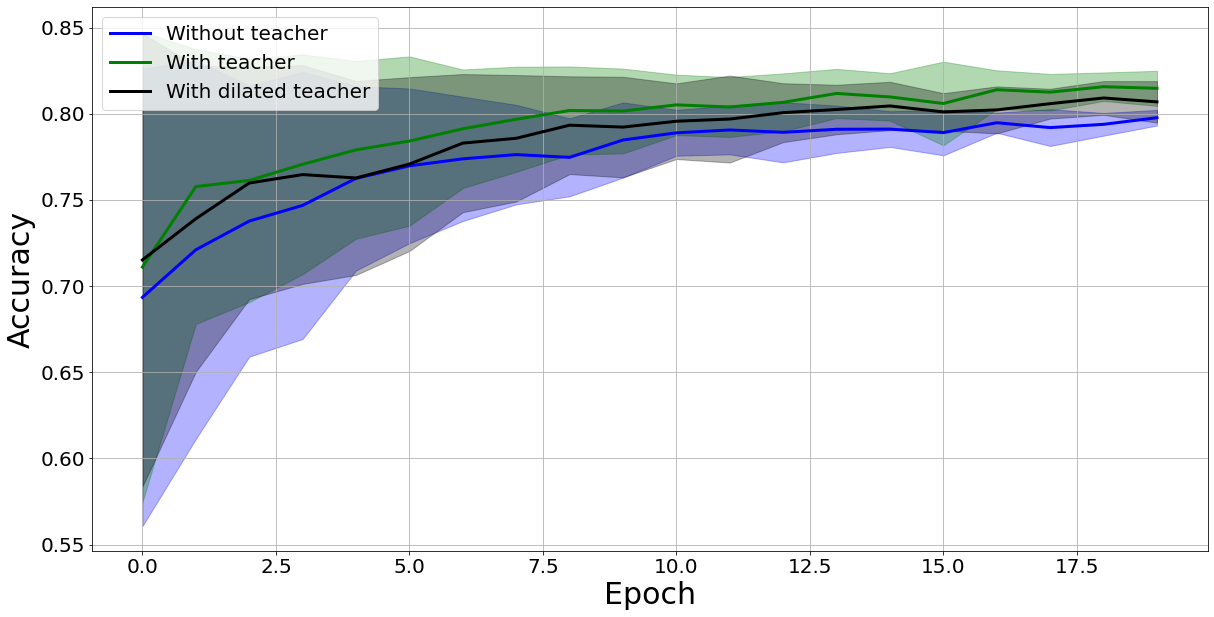
\includegraphics[width=0.5\textwidth]{results/dilation_acc}}
\subfloat[]
{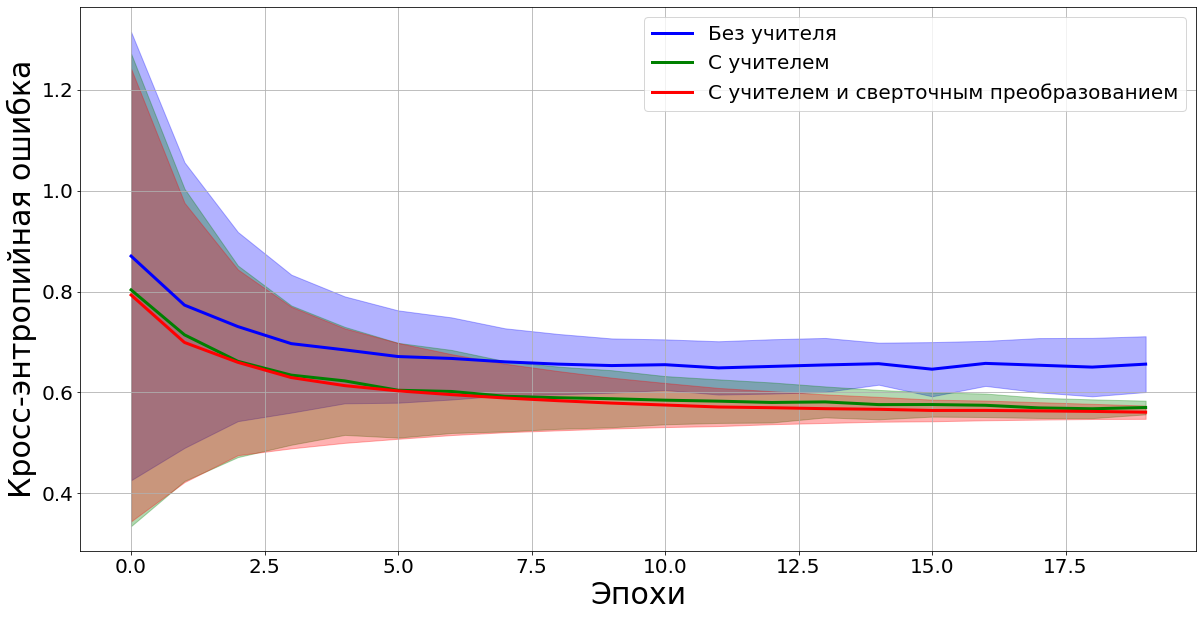
\includegraphics[width=0.5\textwidth]{results/dilation_loss}}\\
\caption{Качество аппроксимации на тестовой выборке a) accuracy; b) CrossEntropyLoss между истинными и предсказанными учеником метками}
\end{figure}

\newpage
\paragraph{Обучение на выборке MNIST.}
Применим к многоресурсному домену преобразование, переводящие изображения одежды из выборки FashionMNIST~\cite{FMNIST} в изображения цифр из выборки MNIST, и обучим на нем модель учителя. Модель ученика обучается на малоресурсном домене.\\
\begin{figure}[h!t]\center
{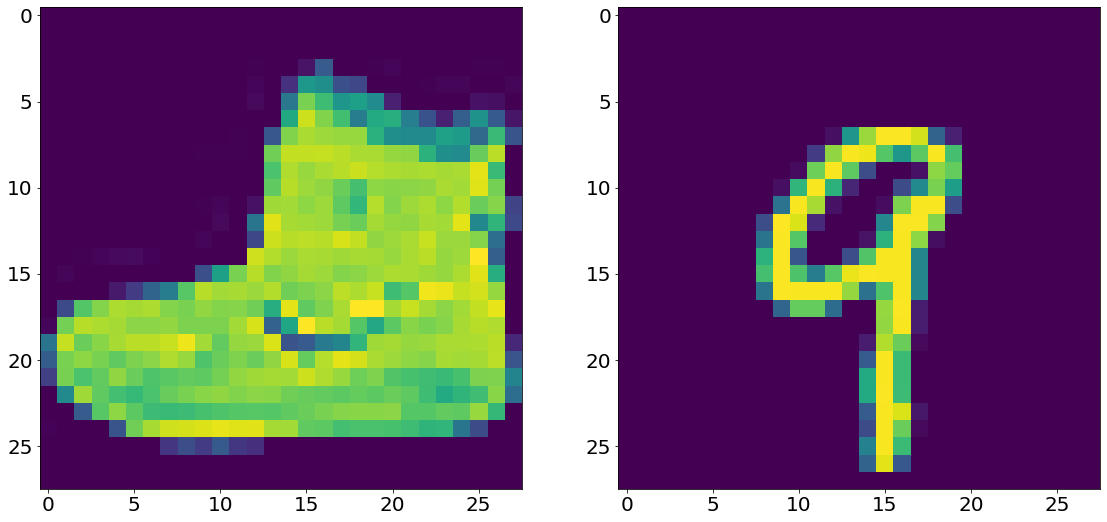
\includegraphics[width=0.5\textwidth]{results/mnist}}
\caption{Сравнение объекта выборки до и после преобразования}
\end{figure}\\
На рис.8а показан график зависимости метрики accuracy на тестовой выборке между истинными метками объектов и вероятностями, предсказанными моделью ученика.\\
На рис.8б показан график зависимости кросс-энтропии на тестовой выборке между истинными метками объектов и вероятностями, предсказанными моделью ученика.\\
На графиках видно, что значения accuracy и CrossEntropyLoss модели, использующей метки учителя на выборке с преобразованием, почти не отличаются от соответствующих значений для модели без учителя.
\begin{figure}[h!t]\center
\subfloat[]
{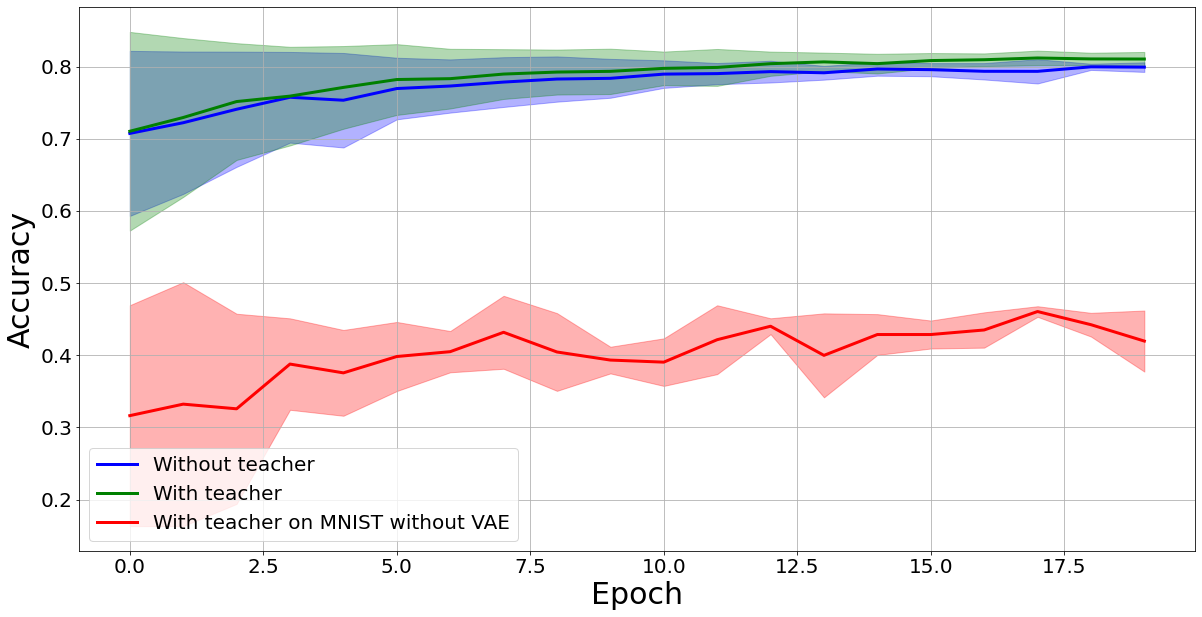
\includegraphics[width=0.5\textwidth]{results/mnist_acc}}
\subfloat[]
{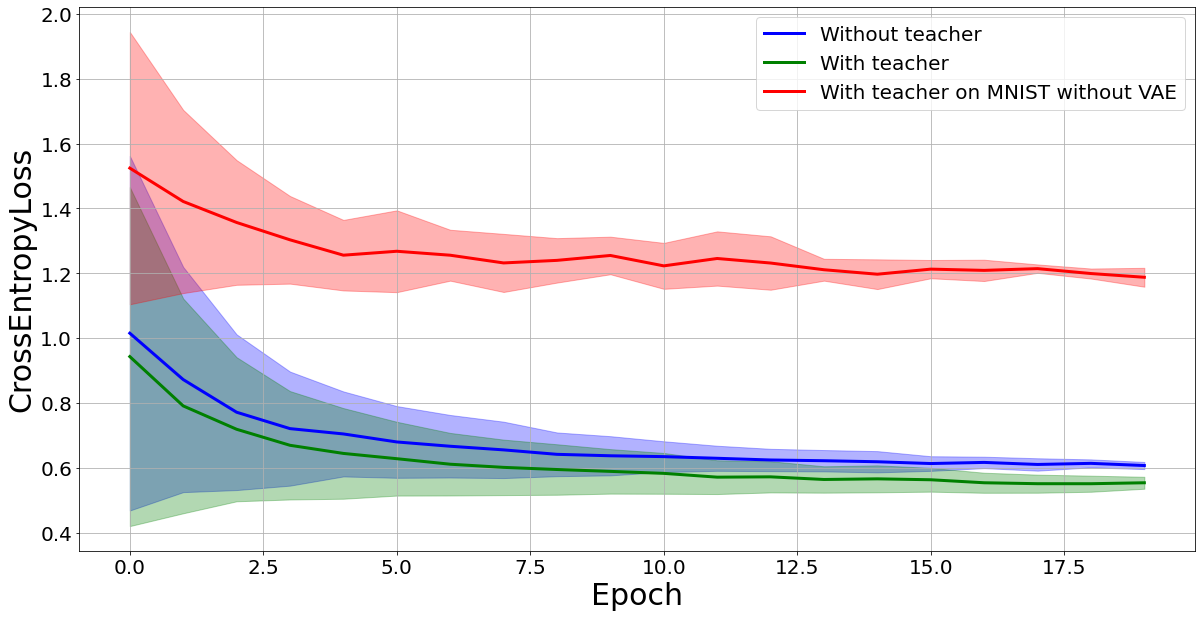
\includegraphics[width=0.5\textwidth]{results/mnist_loss}}\\
\caption{Качество аппроксимации на тестовой выборке a) accuracy; b) CrossEntropyLoss между истинными и предсказанными учеником метками}
\end{figure}



% Библиографические ссылки
\newpage


\begin{thebibliography}{99}
	\bibitem{Hinton2015}
	\textit{Hinton G., Vinyals O., Dean J} Distilling the Knowledge in a Neural Network // NIPS Deep Learning and Representation Learning Workshop. — 2015.
    
    \bibitem{Vapnik2016}
    \textit{D. Lopez-Paz, L. Bottou, B. Schölkopf, V. Vapnik} Unifying distillation and privileged information // ICLR. — 2016.
	
	\bibitem{KimRush2016}
	\textit{Yoon Kim, Alexander M. Rush} Sequence-Level Knowledge Distillation. — 2016.
	
	\bibitem{MDASR}
	\textit{H.Kim, M. Lee, H.Lee, T.Kang, J.Lee, E.Yang, S.Hwang} Multi-domain Knowledge Distillation via Uncertainty-Matching for End-to-End ASR Models. — 2021.
	
	\bibitem{DeepvisDA}
	\textit{Mei Wang, Weihong Deng} Deep Visual Domain Adaptation: A Survey. — 2018.
	
	\bibitem{FMNIST}
    \textit{Xiao H., Rasul K., Vollgraf R.} Fashion-MNIST: a Novel Image Dataset for
    Benchmarking Machine Learning Algorithms. — 2017. https://arxiv.org/abs/1708.07747.
    
    \bibitem{MNIST}
    \textit{LeCun Y., Cortes C.} MNIST handwritten digit database. --- 2010. http://yann.lecun.com/exdb/mnist/
    
    \bibitem{VAE}
    \textit{Diederik P.Kingma, M. Welling} Auto-Encoding Variational Bayes. --- 2014. https://arxiv.org/pdf/1312.6114.pdf
    
    \bibitem{image_to_image}
    \textit{Y. Pang, J. Lin, T. Qin} Image-to-Image Translation: Methods and 
    Applications. --- 2021.
    
    \bibitem{DA}
    \textit{S. Sankaranarayanan, Y. Balaji, A. Jain} Learning from Synthetic Data: Addressing Domain Shift for Semantic Segmentation. --- 2018
    
    \bibitem{Adam}
    \textit{Kingma D., Ba J.} Adam: A Method for Stochastic Optimization // ICLR. — 2015.
    
    \bibitem{UDA}
    \textit{Hongruixuan Chen, Chen Wu, Yonghao Xu, Bo Du} Unsupervised Domain Adaptation for Semantic Segmentation via Low-level Edge Information Transfer. --- 2021.
    
    \bibitem{DA via prompt learning}
    \texit{Chunjiang Ge, Rui Huang, Mixue Xie, Zihang Lai} Domain Adaptation via Prompt Learning. --- 2022.
    
    \bibitem{Model compression}
    \textit{Zhiyuan Wu, Yu Jiang,  Minghao Zhao, Chupeng Cui} Spirit Distillation: A Model Compression Method with Multi-domain Knowledge Transfer
    \bibitem{UDAB}
    \textit{Y.Ganin, V.Lempitsky} Unsupervised Domain Adaptation by Backpropagation. --- 2015
    
    \bibitem{Multi Sourcse Distilling}
    \textit{Sicheng Zhao, Guangzhi Wang, Shanghang Zhang, Yang Gu} Multi-source Distilling Domain Adaptation. --- 2020
    
    \bibitem{DA through distillation}
    \textit{Brady Zhou, Nimit Kalra,  Philipp Krahenbuhl} Domain Adaptation Through Task Distillation. --- 2020

	
\end{thebibliography}



\end{document}